\documentclass[a4paper,12pt]{article}

\usepackage[scaled=0.92]{helvet}

\usepackage[colorlinks=true, linkcolor=blue]{hyperref}

\usepackage[english]{babel}
\selectlanguage{english}

\usepackage{microtype}
\usepackage{graphicx}
\usepackage{wrapfig}
\usepackage{enumitem}
\usepackage{amsmath}
\usepackage{index}
\usepackage[utf8]{inputenc}
\usepackage[svgnames]{xcolor}
\usepackage{url}
\usepackage{hyperref}
\usepackage{float}
\usepackage{longtable}
\usepackage[toc]{glossaries}

\begin{document}

\begin{titlepage}

\begin{center}
\vspace*{-1.2in}
\begin{figure}[htb]
\begin{center}

\includegraphics[width=10cm]{Concordia_logo.png}
\end{center}
\end{figure}
\begin{Large}
\vspace*{0.3in}
\textbf{Project Report} \\
\end{Large}
\vspace*{0.1in}
\begin{Large}
For\\
\end{Large}
\vspace*{0.1in}

\begin{Large}
\textbf{Deliverable 2} \\
\end{Large}
\vspace*{0.1in}

\begin{Large}
\textbf{iGo} \\
\end{Large}
\vspace*{0.3in}

\begin{large}
\textbf{Submitted By: TEAM R} \\[1.0 cm]
\vspace*{0.1in}
Anant Bir Singh\\
Prabhjot Singh\\
Piyush Singla\\
Parth Sonani\\
Shivam Dipak Soni\\
\vspace*{0.2in}
\textbf{Submitted to}\\
\vspace*{0.1in}
Prof. Pankaj Kamthan\\
\vspace*{0.3in}

\begin{Large}
\textbf{SOEN 6461 - Software Design Methodologies} \\
\vspace*{0.2in}
\textbf{Concordia University, Montreal, QC}
\end{Large}

\end{large}
\end{center}
\end{titlepage}


\newcommand{\CC}{C\nolinebreak\hspace{-.05em}\raisebox{.4ex}{\tiny\bf +}\nolinebreak\hspace{-.10em}\raisebox{.4ex}{\tiny\bf +}}
\def\CC{{C\nolinebreak[4]\hspace{-.05em}\raisebox{.4ex}{\tiny\bf ++}}}

\tableofcontents
\newpage
\section{High level solution domain model}
\subsection{CRC Model for iGo}
A Class Responsibility Collaborator (CRC) model is a collection of standard
index cards that have been divided into three sections, as
\begin{itemize}
  \item A class represents a collection of similar objects.
  \item a responsibility is something that a class knows or does.
  \item a collaborator is another class that a class interacts with to fulfill its
responsibilities
\end{itemize}
Below are the CRC cards for the classes which relate to iGo.
\begin{center}
  \makebox[\textwidth]{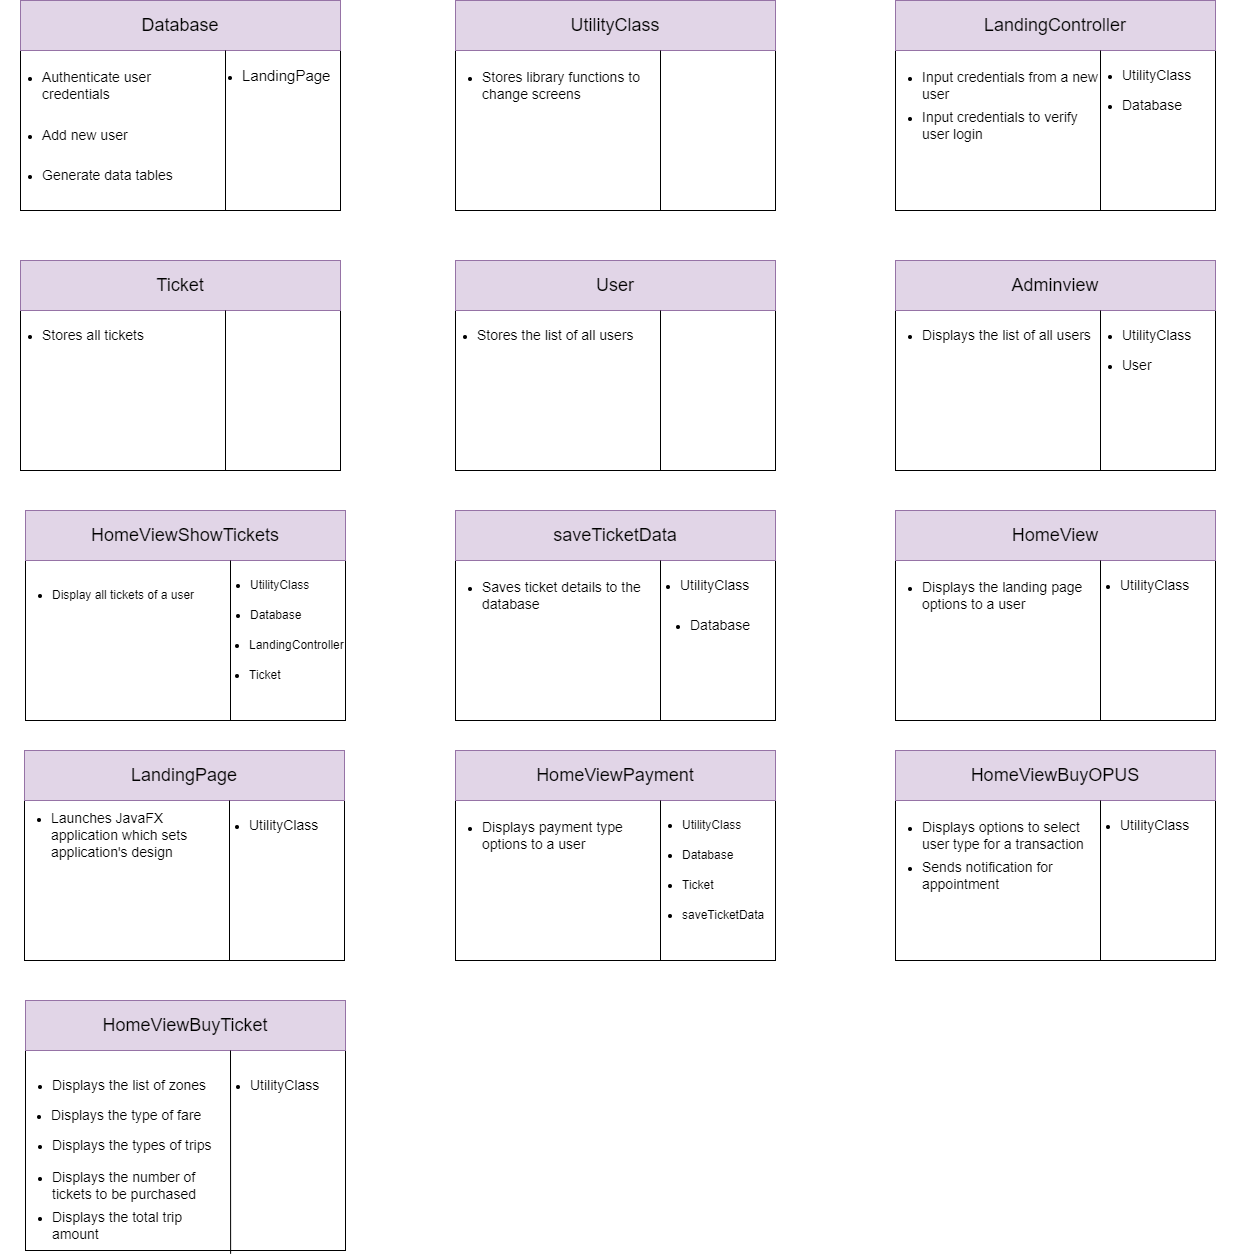
\includegraphics[width=\linewidth]{CRC_iGo.png}}
\caption{CRC Card Model of iGo}
\end{center}

\newpage
\section{Low level solution domain model}
\subsection{Structural Design Model}
Structural design model refers to a type of model that represents the static structure of a system, including the components, their relationships, and the constraints between them. It is used to specify the architecture of a system and to ensure that the components are properly integrated and interact with each other as intended. \\ \par

UML class diagram is a type of structural design model that represents the static structure of a system in terms of its classes, their attributes, methods, and relationships. Class diagrams are commonly used in object-oriented programming to represent the classes that make up a system and their relationships to each other.\\ \par

Below given diagram is the UML class diagram of iGo which consists of all the classes and the relations between them. \\
\begin{center}
  \makebox[\textwidth]{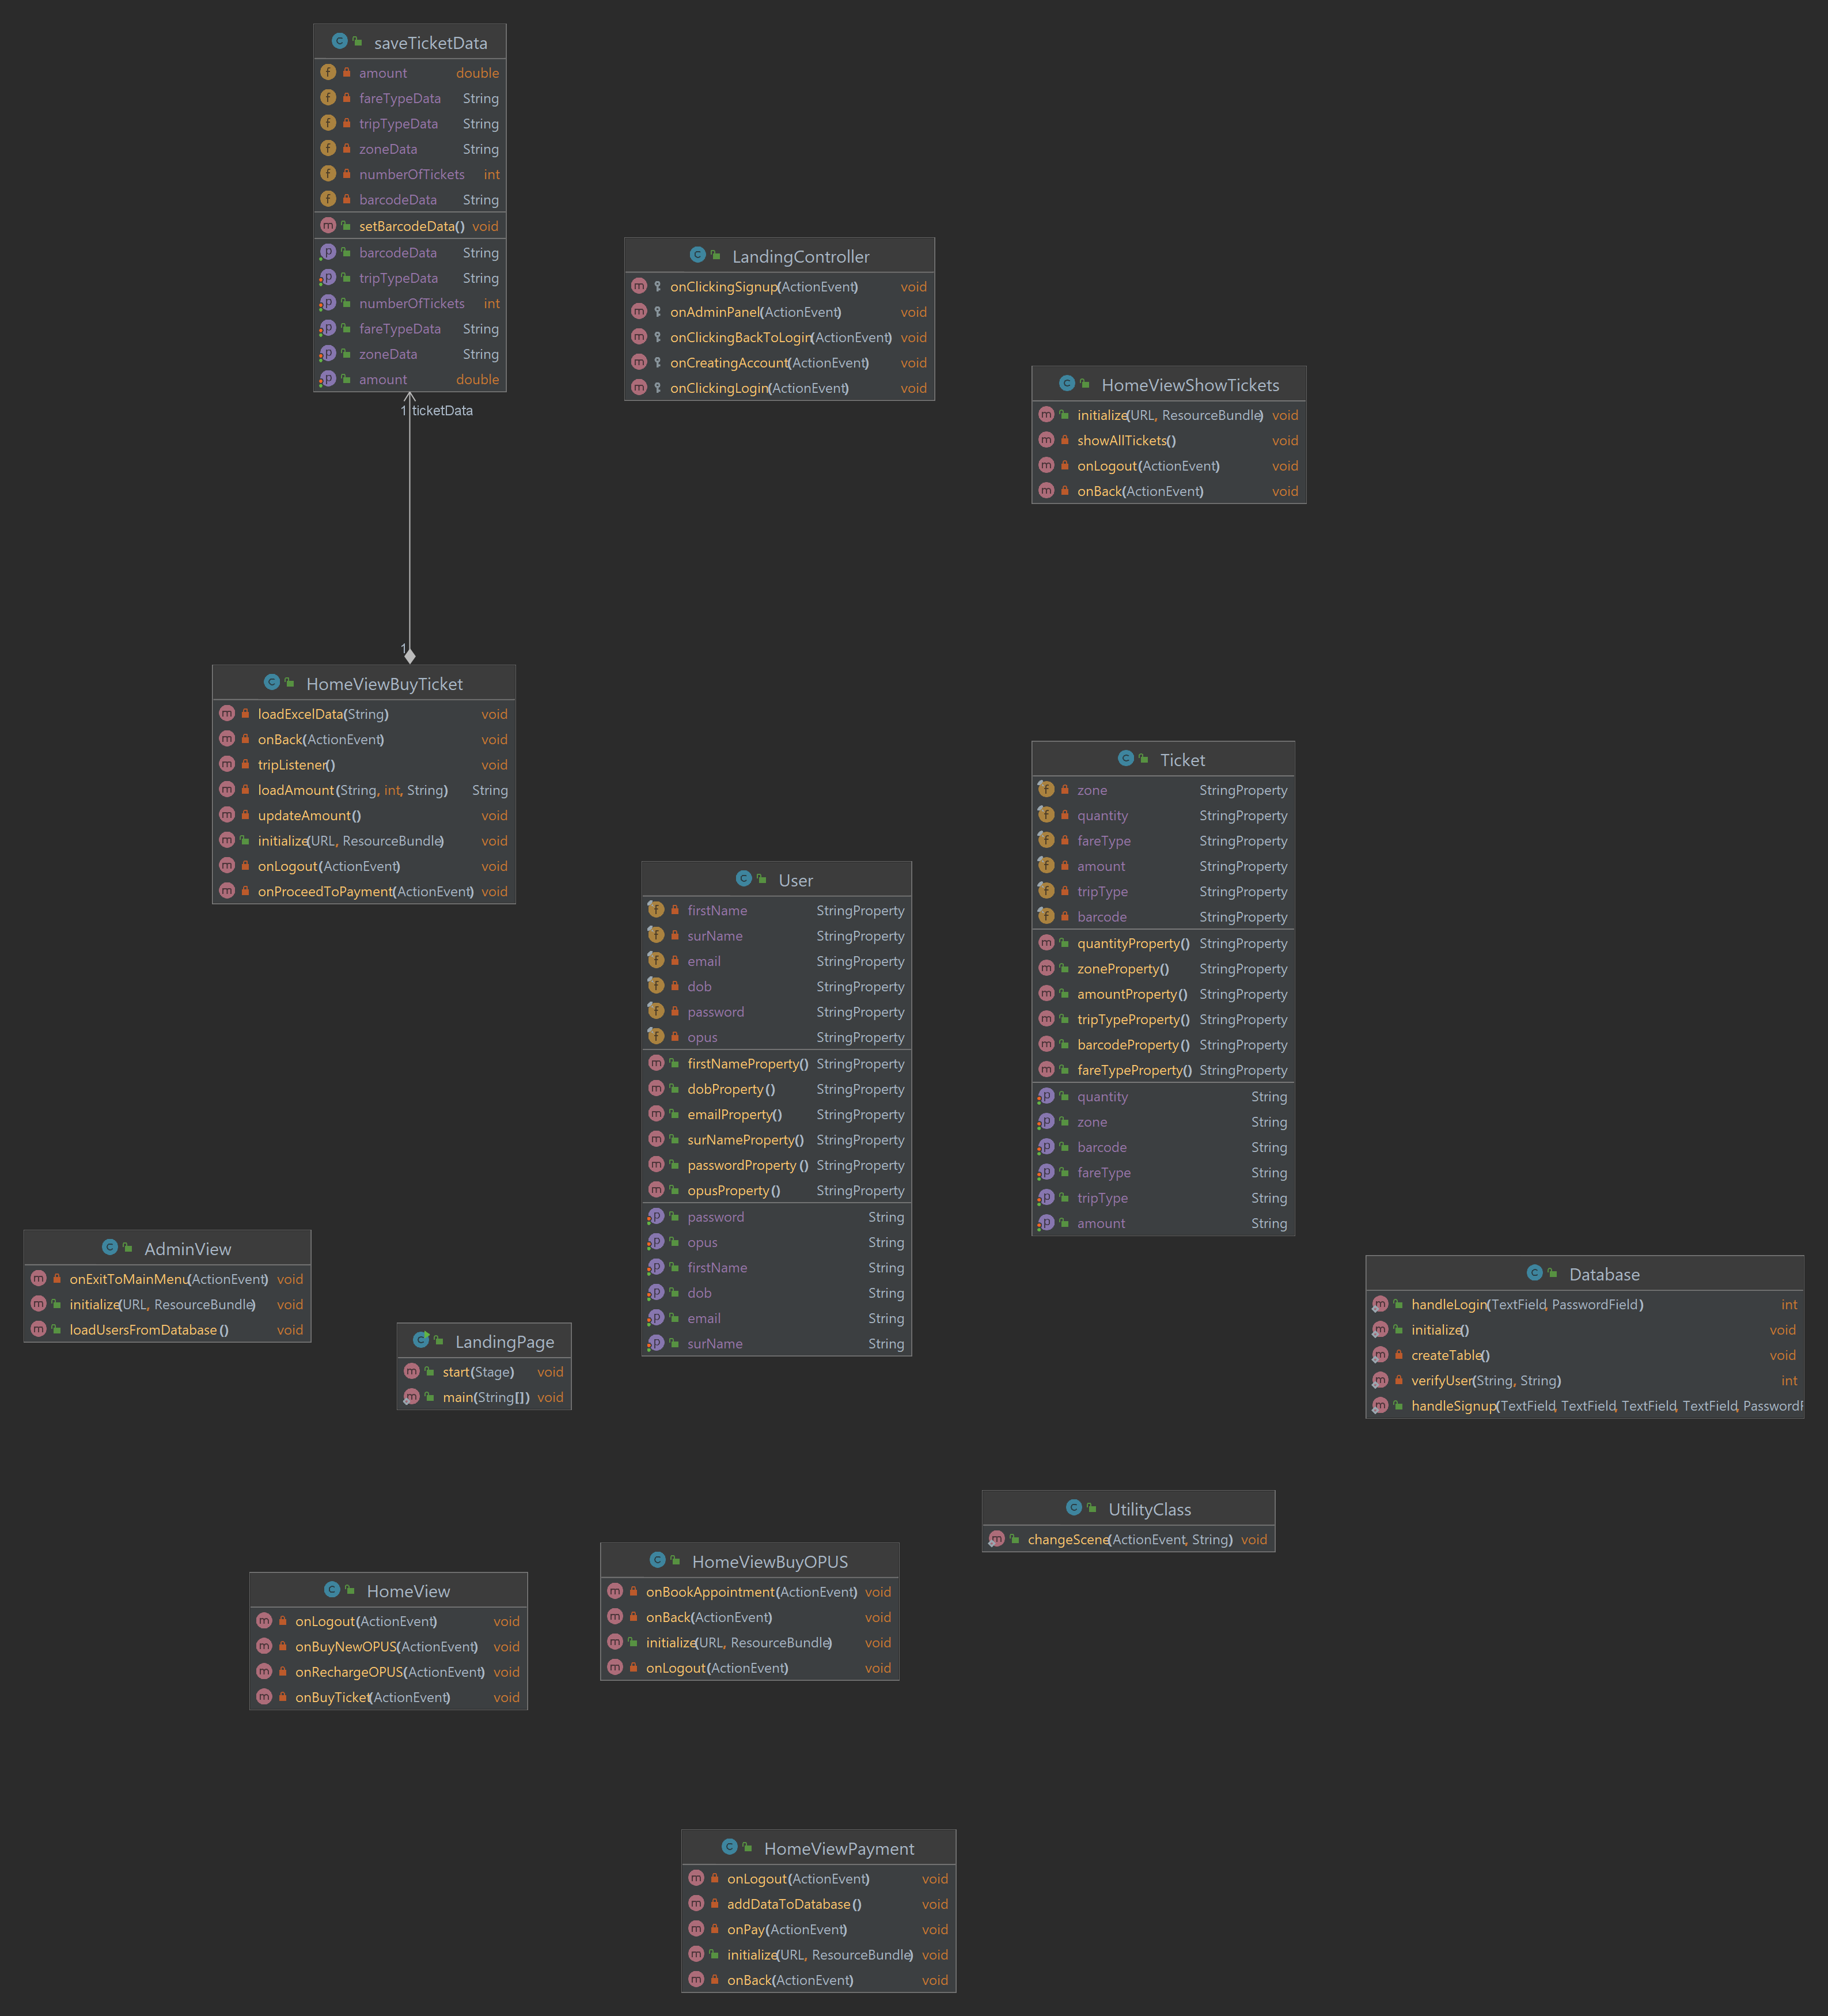
\includegraphics[width=\linewidth]{UML_class_diagram.png}}
\caption{UML class diagram of iGo}
\end{center}

\subsection{Behavioral Design Model}
Behavioral design model refers to a type of model that represents the dynamic behavior of a system, including the interactions between its components and the flow of data and control between them. It is used to specify the behavior of a system and to ensure that it meets the desired functional requirements.\\ \par

Sequence diagrams are a type of behavioral design model that represent the interactions between the objects or components of a system over time. They show the sequence of events that occur in a particular scenario or use case, including the messages that are passed between the objects and the order in which they are processed. \\ \par

The following sections describes the 5 sequence diagrams which are the processes followed in the iGo.

\begin{center}
  \makebox[\textwidth]{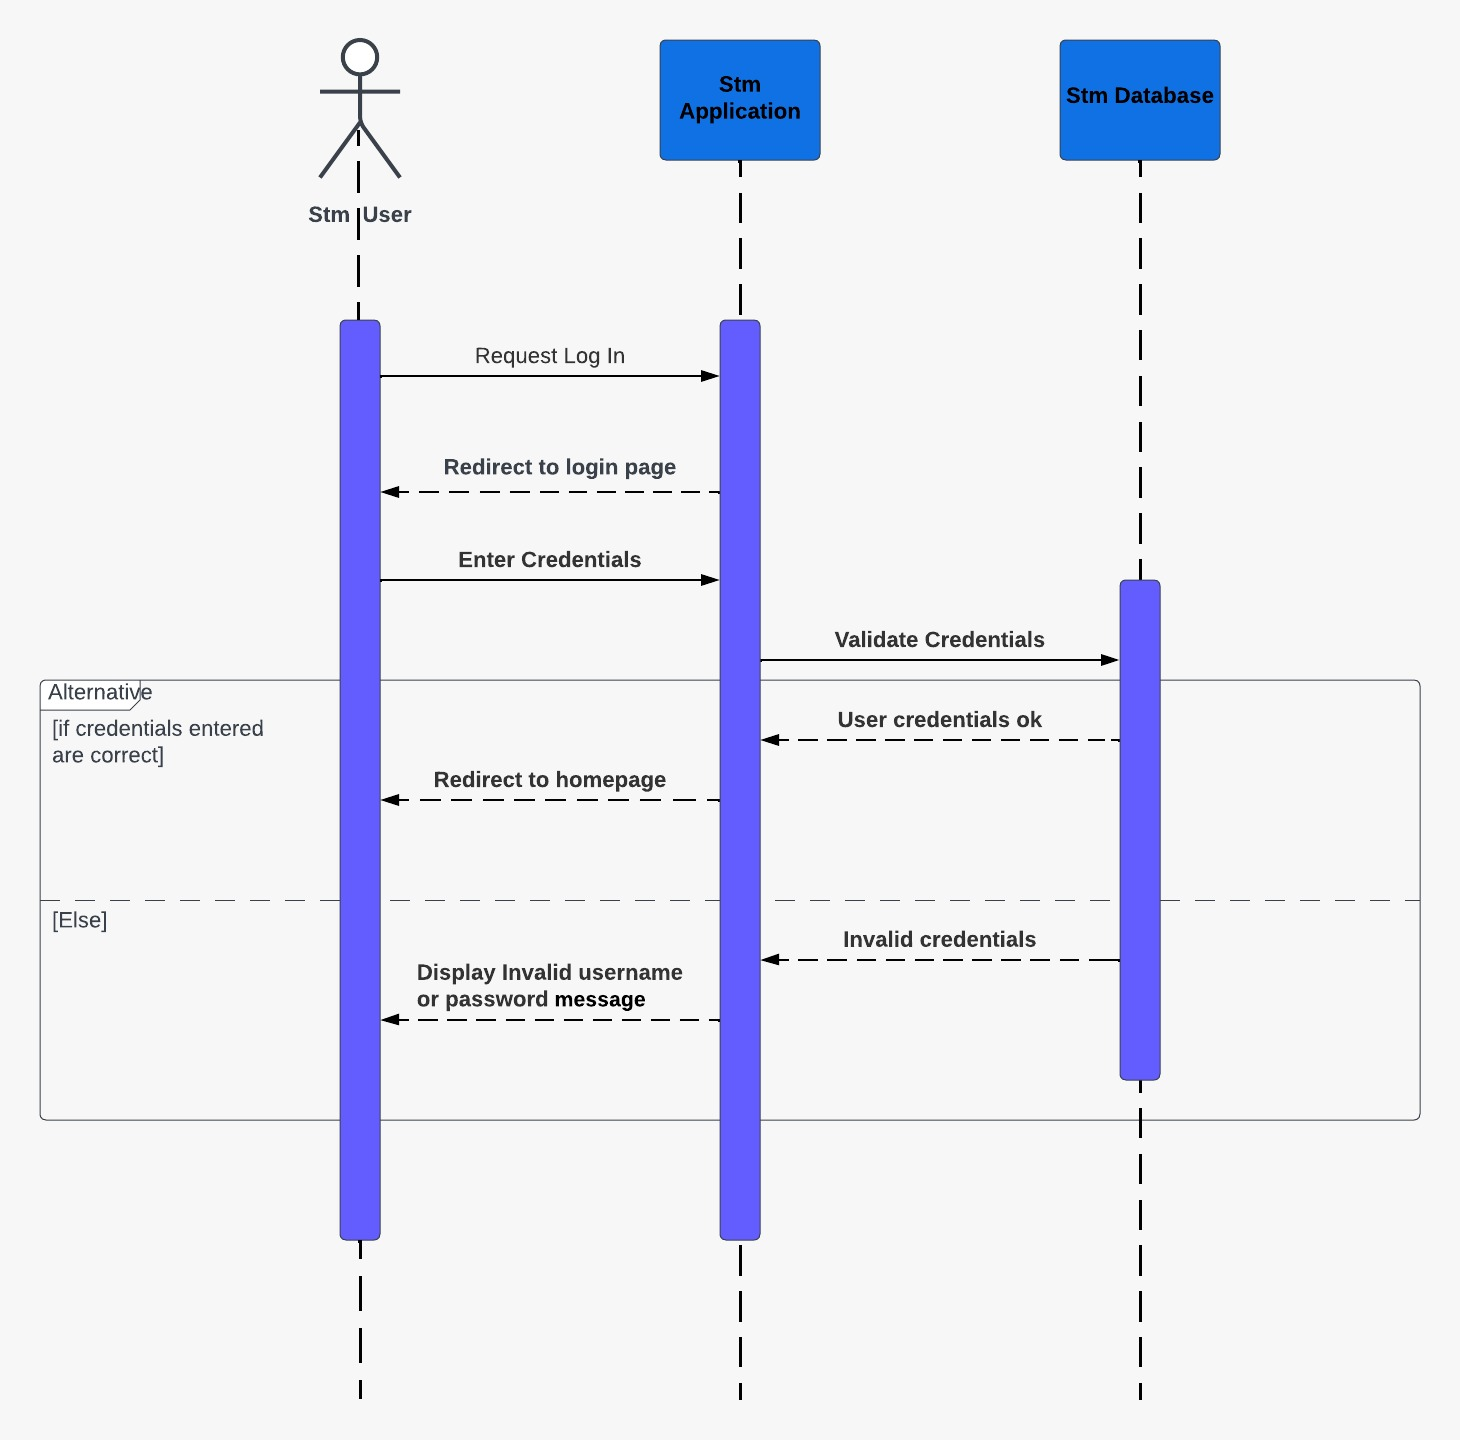
\includegraphics[width=\linewidth]{Login.jpeg}}
\caption{1. UML sequence diagram for login}
\end{center}

\begin{center}
  \makebox[\textwidth]{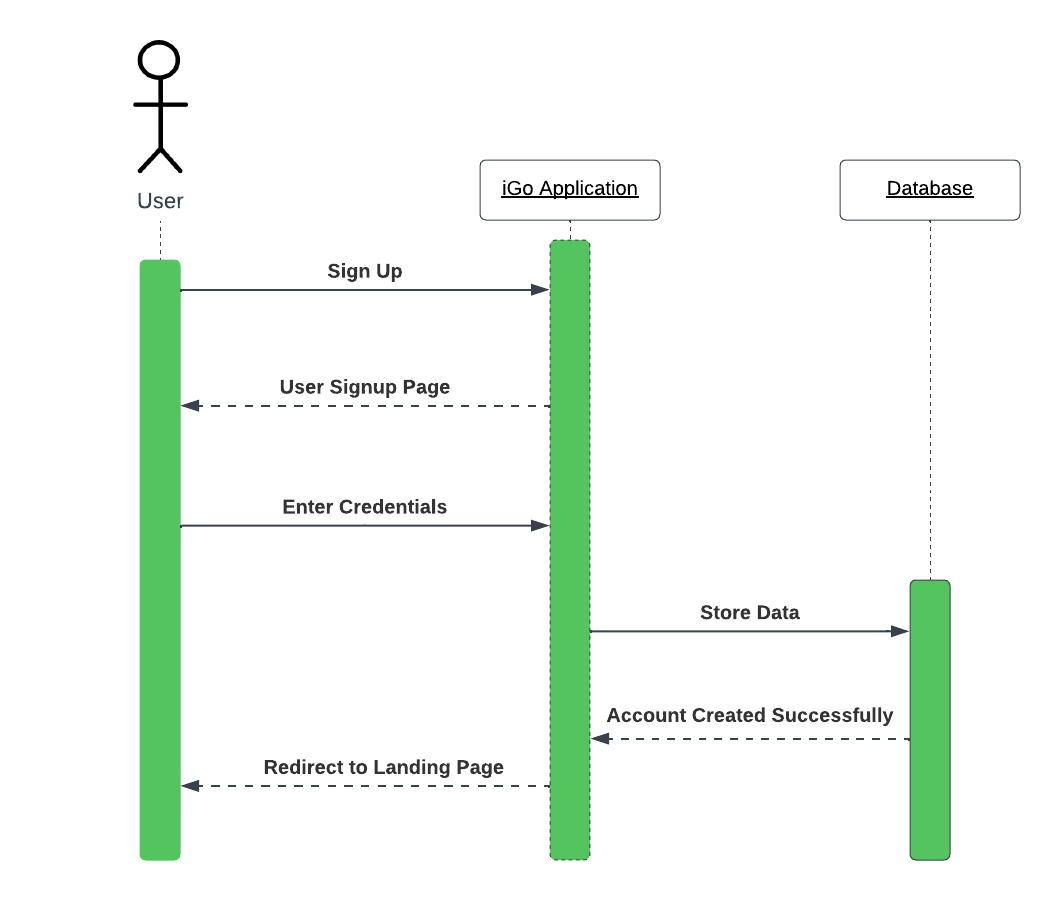
\includegraphics[width=\linewidth]{Signup.png}}
\caption{2. UML sequence diagram for signup}
\end{center}

\begin{center}
  \makebox[\textwidth]{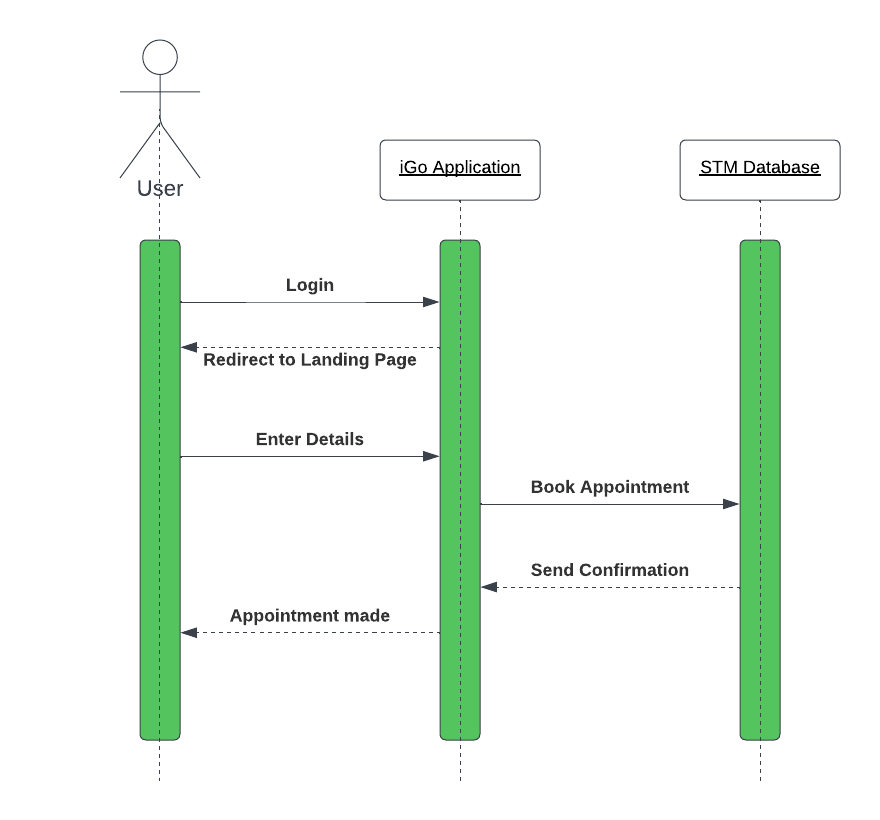
\includegraphics[width=\linewidth]{Buy_New_OPUS.png}}
\caption{3. UML sequence diagram to buy new OPUS card}
\end{center}

\begin{center}
  \makebox[\textwidth]{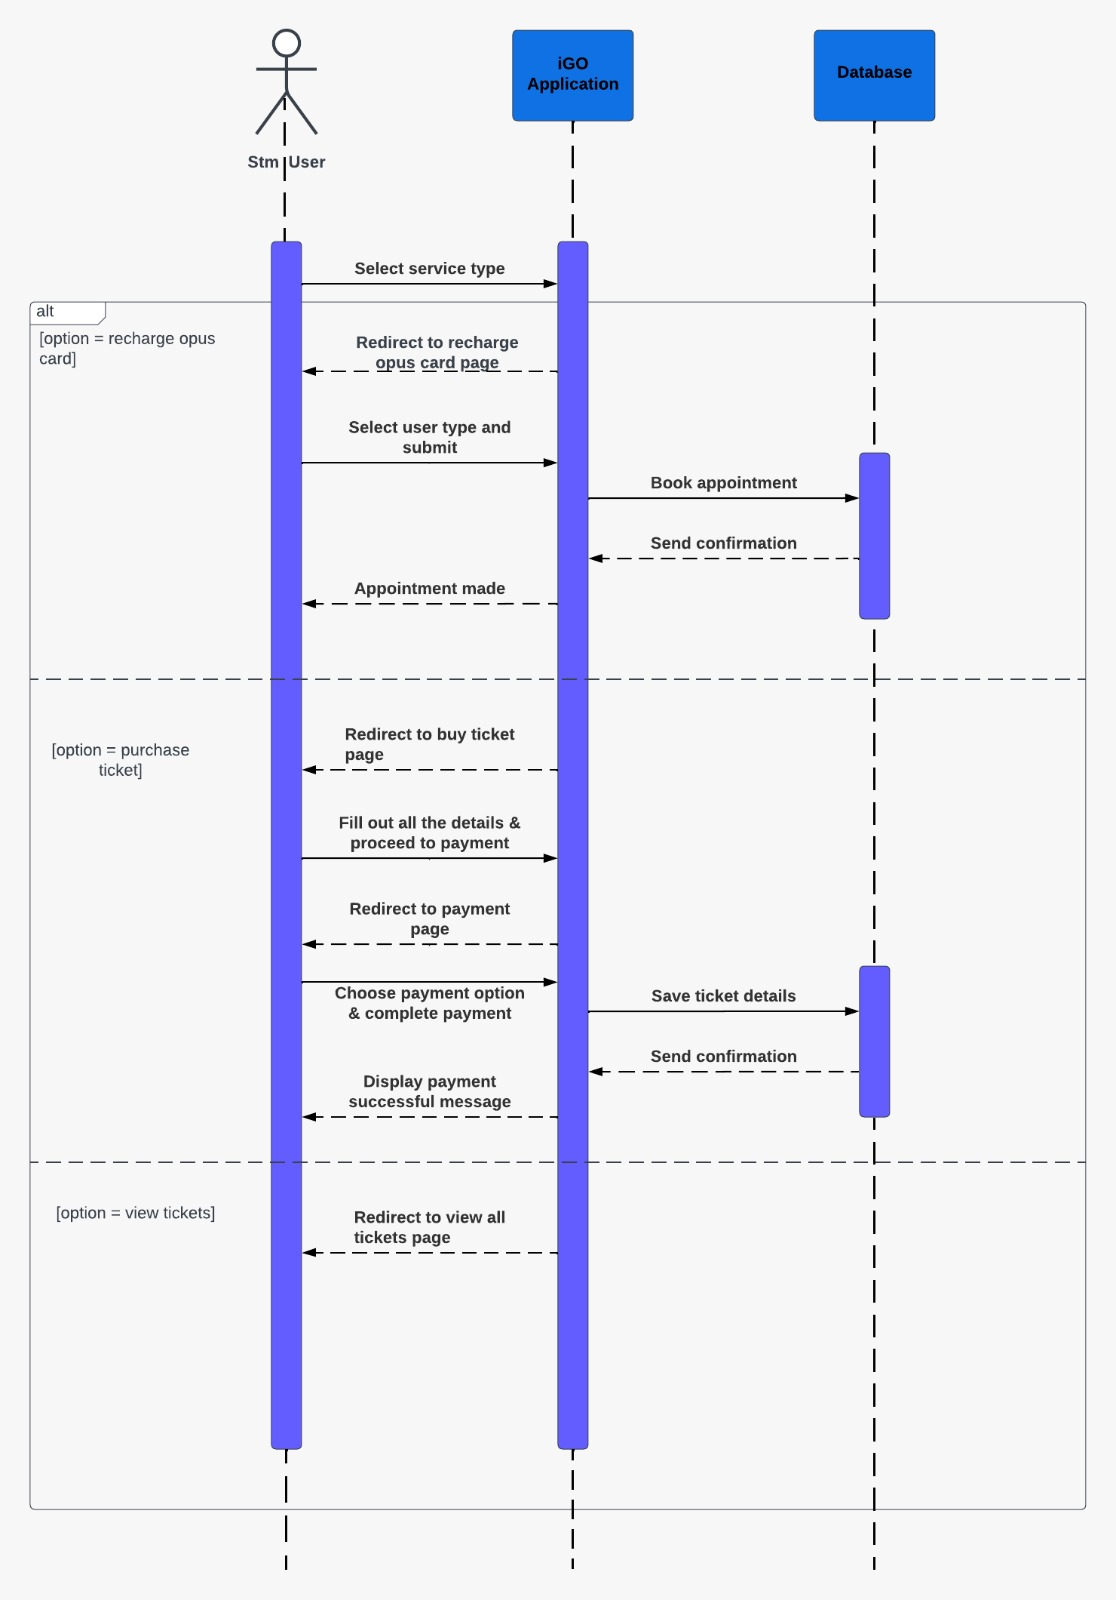
\includegraphics[width=\linewidth]{Recharge_Purchase_View.jpeg}}
\caption{4. UML sequence diagram for buying new opus, selecting ticket and viewing ticket}
\end{center}

\begin{center}
  \makebox[\textwidth]{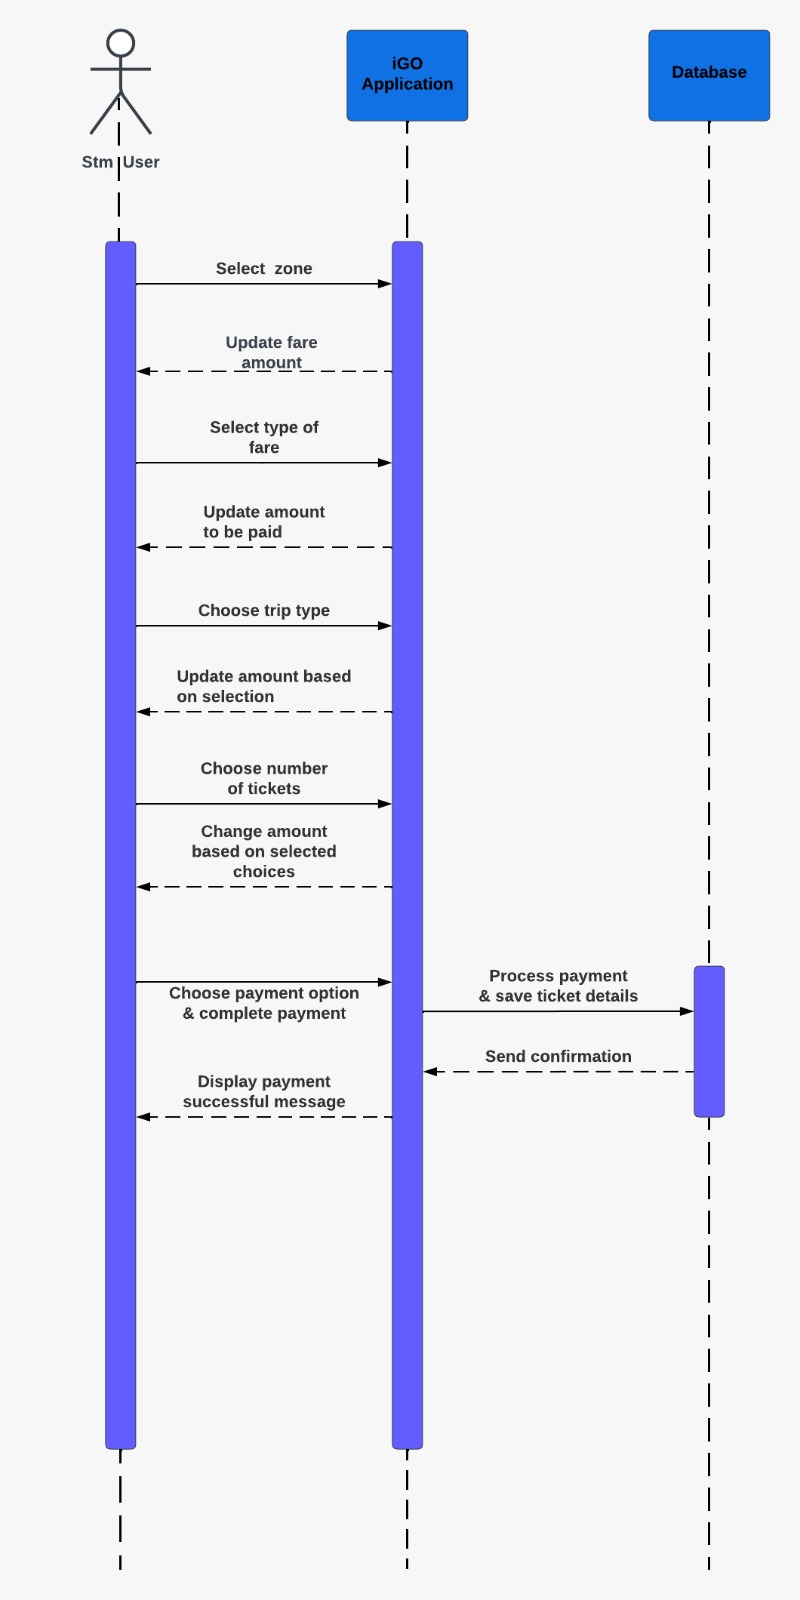
\includegraphics[height=20cm]{Trip_payment.jpg}}
\caption{5. UML sequence diagram for selecting the trip and payment}
\end{center}

\newpage
\section{iGo - Javafx code}
\subsection{GitHub repository link : \href{https://github.com/singlapiyush1/SDM-Project/tree/main/Code}{iGo}}

\subsection{Programming Style and GUI}
The GUI application for the iGo is developed using the java programming language. The javafx sdk is used for developing this application. \\ \par
The java program uses Procedural programming style with object oriented programming practice.

\subsection{Program flow}
The Program flow section of this report provides a brief description of the flow of control within the software system. The sequence of the program is as follow:
\begin{itemize}[noitemsep]
    \item The program first launches the login page.
    \item If the user is registered then the user can login to the application, otherwise the user can proceed to signup page.
    \item The user can add all the necessary details such as "First name", "Surname", "Email", "Password", "OPUS serial number"(optional), "Date of Birth" and successfully signup.
    \item The email is considered as the username with which the user can log in the application
    \item After signing up or logging in the application the user is taken to the home page where the user has 3 main options
    \begin{enumerate}
        \item Buy new opus
        \begin{itemize}
            \item Clicking on this option leads to the screen where the user can book appointment for buying the discounted opus card.
            \item After selecting the appropriate option and clicking on the book appointment the user is prompted with a message about an email being sent to user with appointment details
        \end{itemize}
        \item Buy ticket
        \begin{itemize}
            \item Clicking on this option leads to screen where the user is given option to select the zone for the ticket (ex. A, A & B,...), select fare type (ex. Regular, 65 and over,...), select trip type (ex. 1 trip, 2 trips,...), and number of tickets.
            \item After the user has successfully selected the options the user can click on the proceed payment button.
            \item On clicking the proceed payment the user is shown option to select the payment method and payment is done.
        \end{itemize}
        \item View my tickets
        \begin{itemize}
            \item On clicking this option all the purchased tickets of the logged in user can be seen by the user.
        \end{itemize}
    \end{enumerate}
    \item There is one more option "Admin Panel" which shows how many users are registered on the application.
\end{itemize}

\subsection{Assumptions or limitations in program}
There are certain assumptions in the program which are as follow
\begin{itemize}[noitemsep]
    \item The database is a local database, the user cannot login remotely.
    \item The program cannot validate the OPUS.
    \item The data for the zone, fare, trip are static (if stm changes data for this we need to also update it in files)
    \item The payment method is assumed to be a 3rd party.
\end{itemize}

\newpage
\section{Testing iGo}
\par
The following section will demonstrate the working of the application iGo along with it's functionalities through the use of images.
\subsection{Registering the user}

\begin{center}
  \makebox[\textwidth]{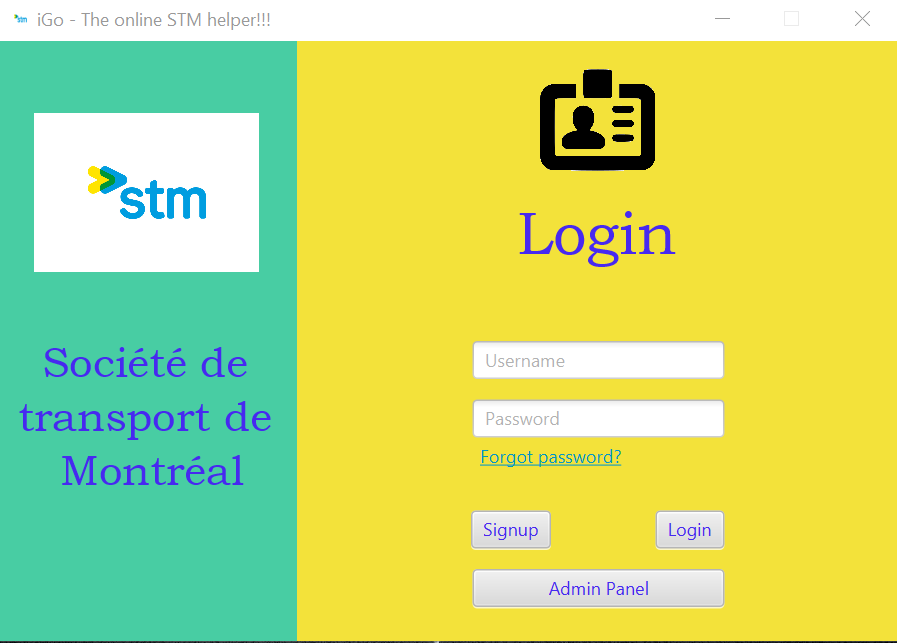
\includegraphics[width=\linewidth]{LoginPage.png}}
\caption{1. The landing page of the application}
\end{center}

\begin{center}
  \makebox[\textwidth]{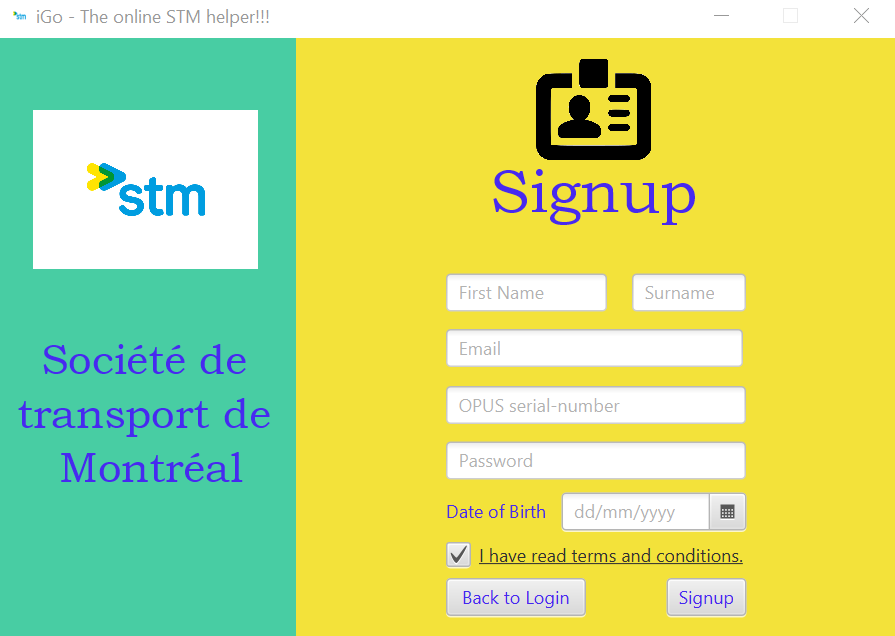
\includegraphics[width=\linewidth]{SignupPage.png}}
\caption{2. Signup page of the application}
\end{center}

\begin{center}
  \makebox[\textwidth]{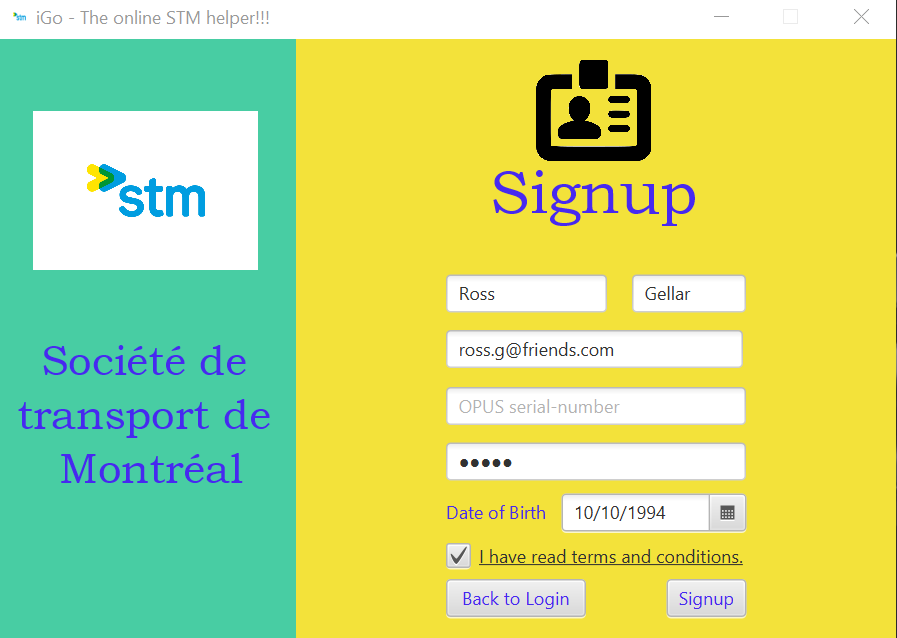
\includegraphics[width=\linewidth]{UserSigningUp.png}}
\caption{3. User filling up the information for signing on}
\end{center}

\subsection{User home}
\begin{center}
  \makebox[\textwidth]{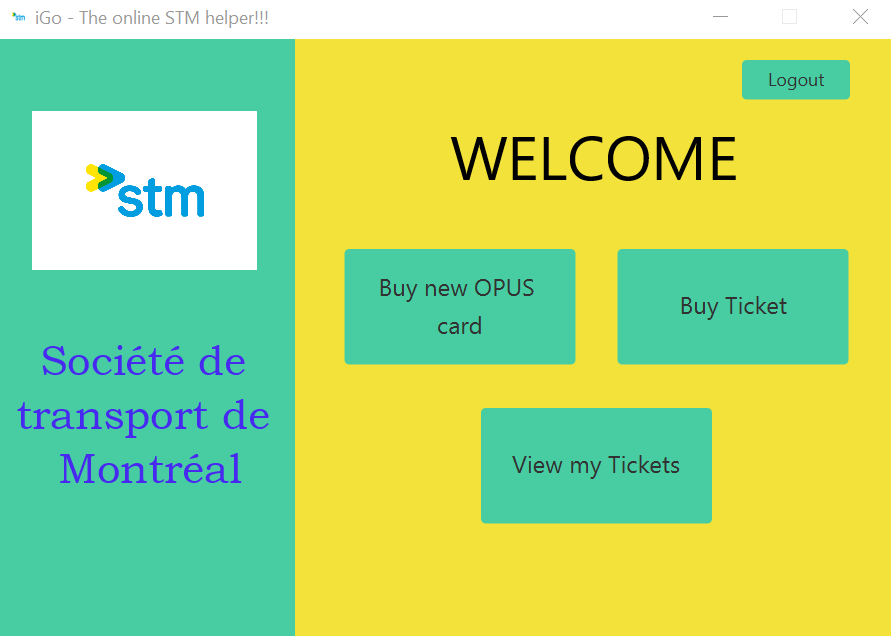
\includegraphics[width=\linewidth]{UserHomePage.png}}
\caption{1. Homepage for user after signing in or logging in application}
\end{center}

\subsubsection{Buy new OPUS card}
\begin{center}
  \makebox[\textwidth]{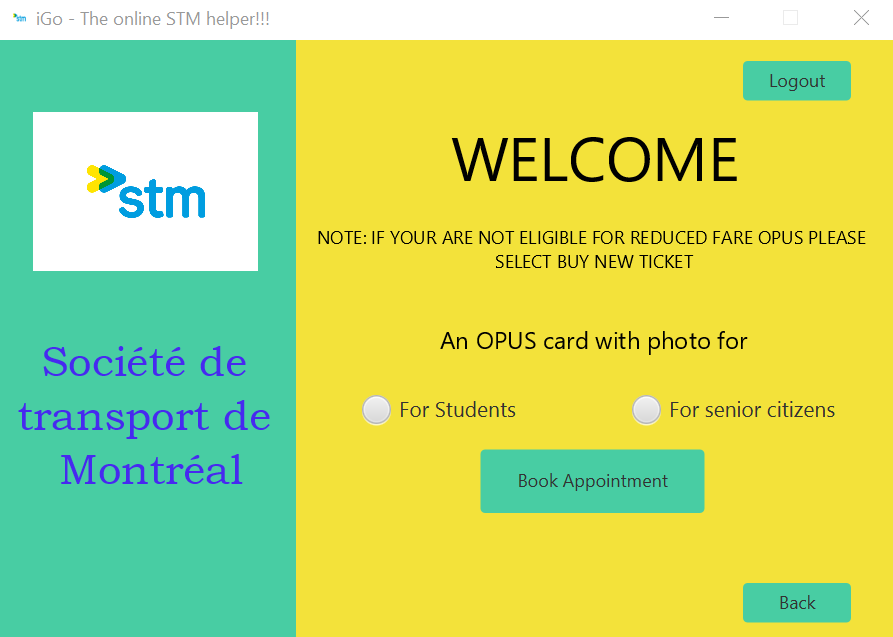
\includegraphics[width=\linewidth]{BuyNewOpusPage.png}}
\caption{2. Option to buy a new OPUS card}
\end{center}

\begin{center}
  \makebox[\textwidth]{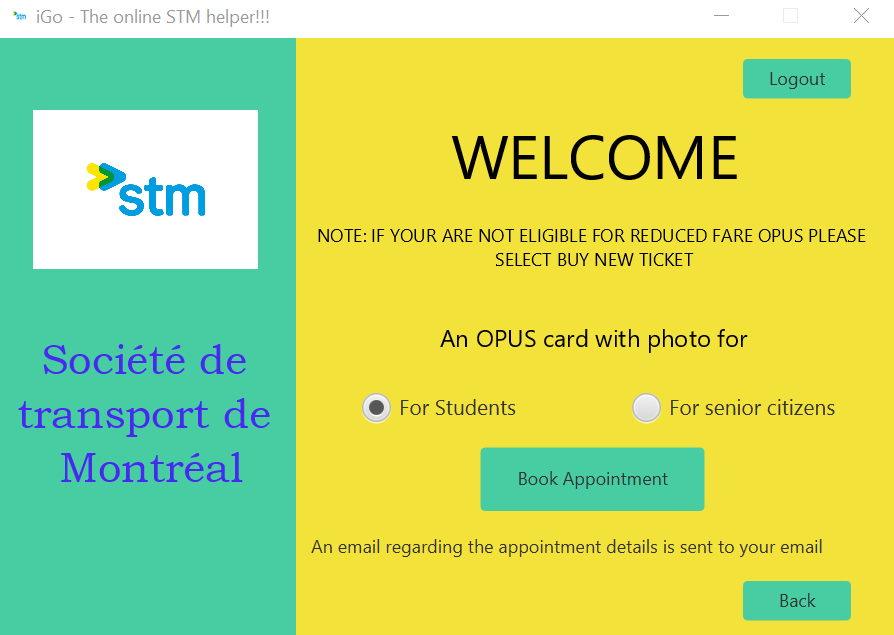
\includegraphics[width=\linewidth]{BuyNewOpusEmailNotification.png}}
\caption{3. Notification after selecting the right option}
\end{center}

\subsubsection{Buy Ticket}
\begin{center}
  \makebox[\textwidth]{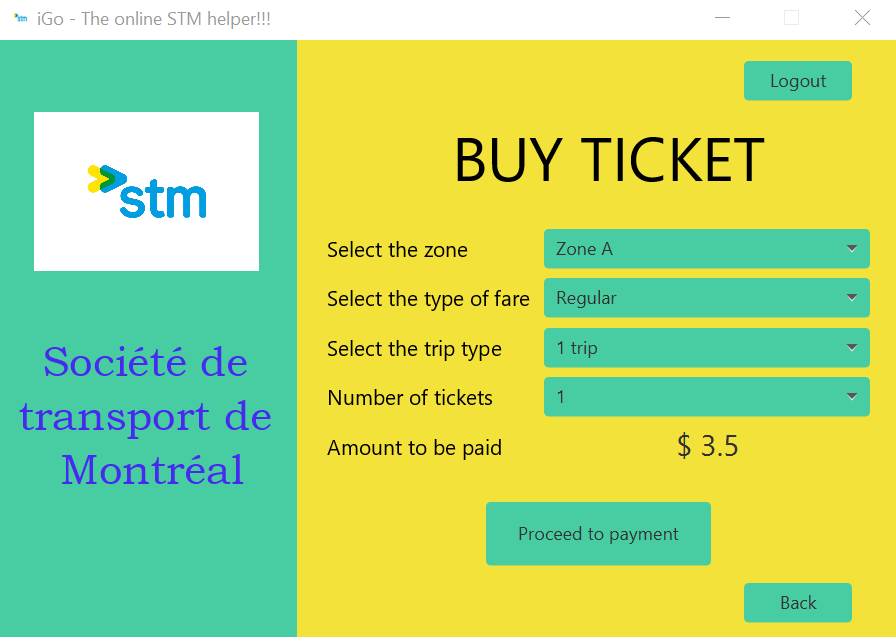
\includegraphics[width=\linewidth]{BuyTicketPage.png}}
\caption{4. Page to select different types of trips and amount of tickets}
\end{center}

\begin{center}
  \makebox[\textwidth]{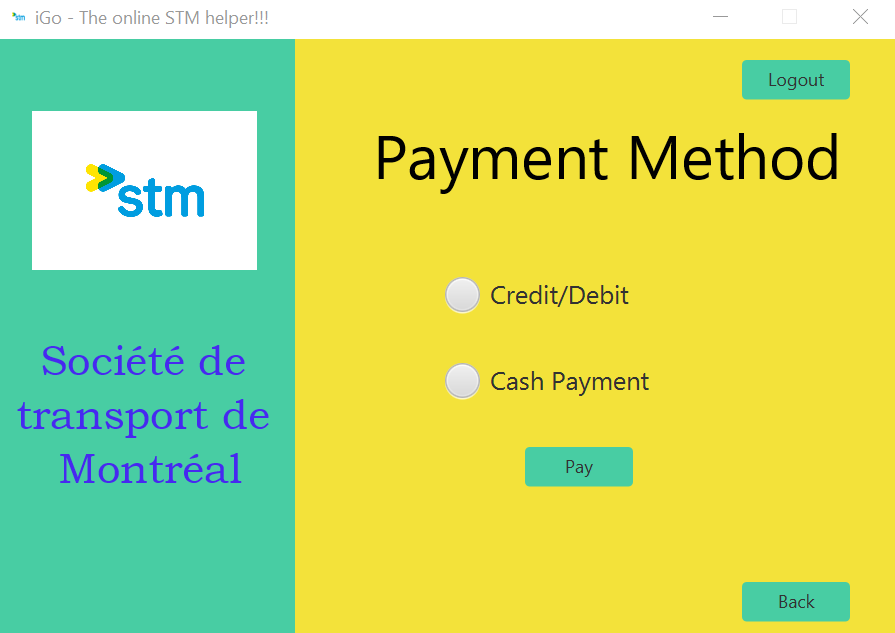
\includegraphics[width=\linewidth]{PaymentMethodPage.png}}
\caption{5. The payment method page for buying ticket}
\end{center}

\begin{center}
  \makebox[\textwidth]{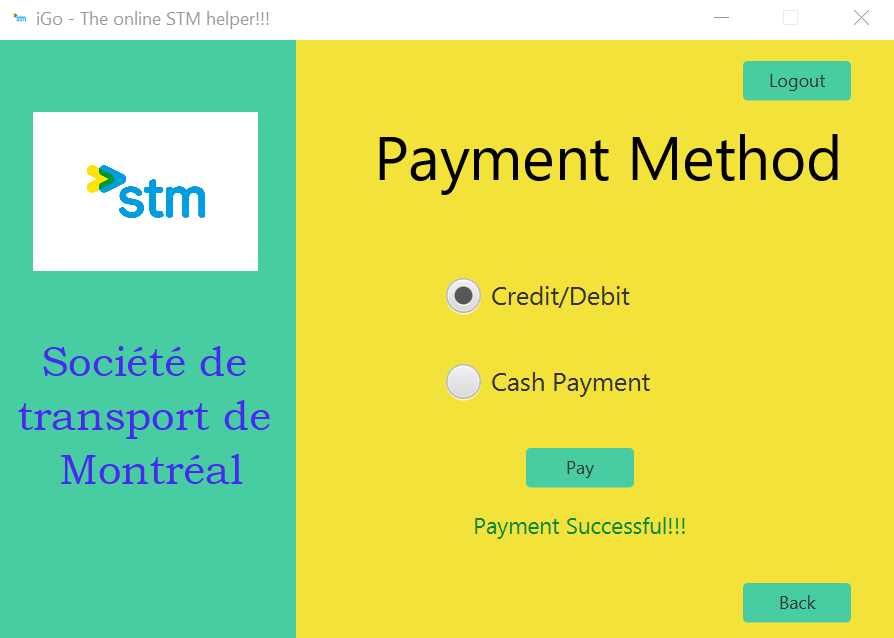
\includegraphics[width=\linewidth]{PaymentSuccessMessage.png}}
\caption{6. Payment success message}
\end{center}

\subsubsection{View my tickets}
\begin{center}
  \makebox[\textwidth]{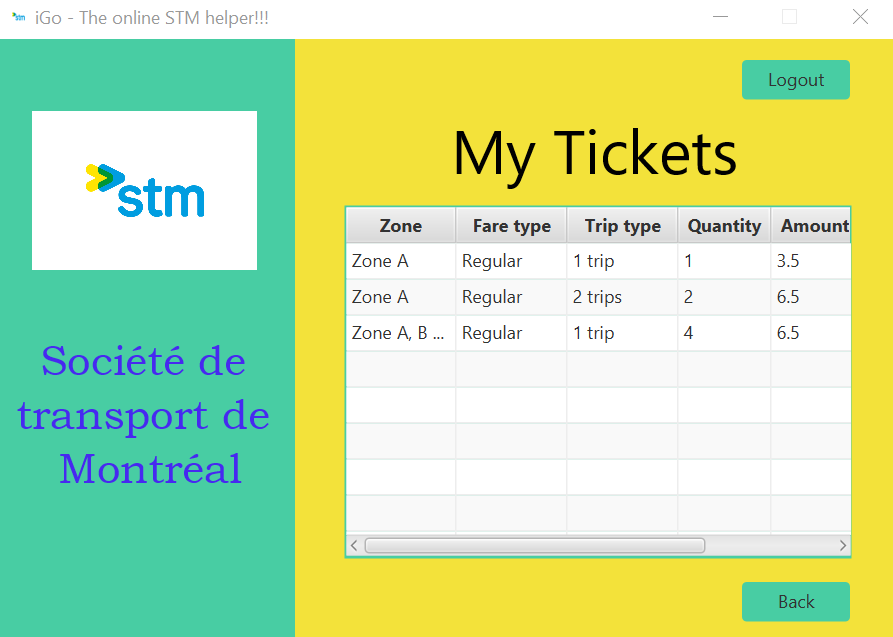
\includegraphics[width=\linewidth]{UserShowTickets.png}}
\caption{1. Page to show all the tickets purchased by the logged in user}
\end{center}

\subsection{Admin panel}
\begin{center}
  \makebox[\textwidth]{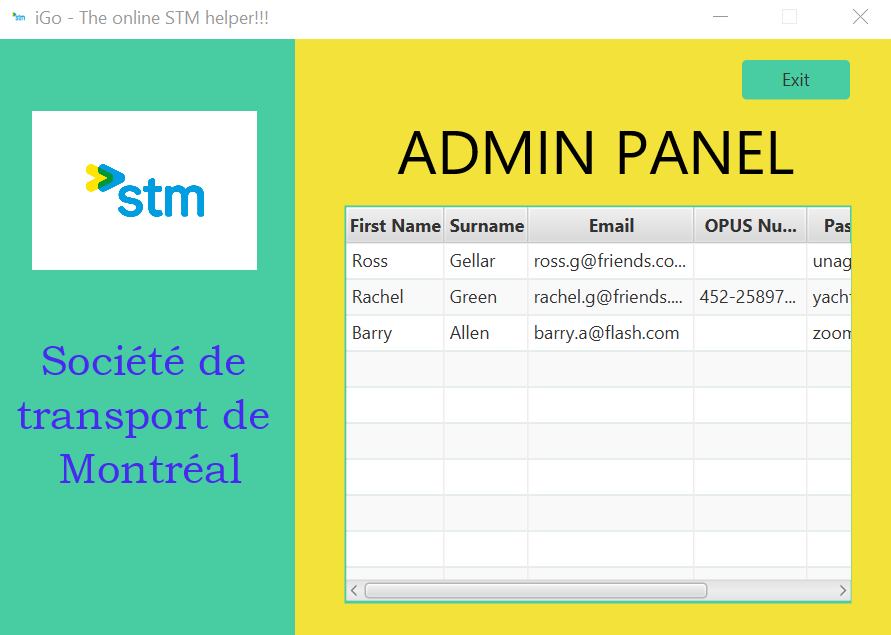
\includegraphics[width=\linewidth]{AdminPanel.png}}
\caption{1. Admin panel to view all the available users}
\end{center}

\subsection{Invalids or Exceptions}
\begin{center}
  \makebox[\textwidth]{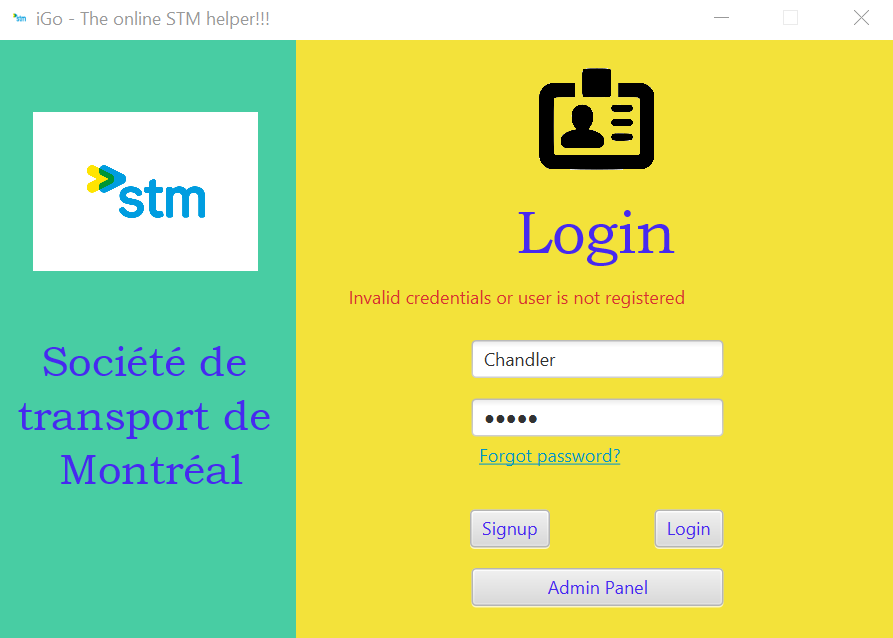
\includegraphics[width=\linewidth]{InvalidLogin.png}}
\caption{1. Unregistered user trying to log in}
\end{center}

\begin{center}
  \makebox[\textwidth]{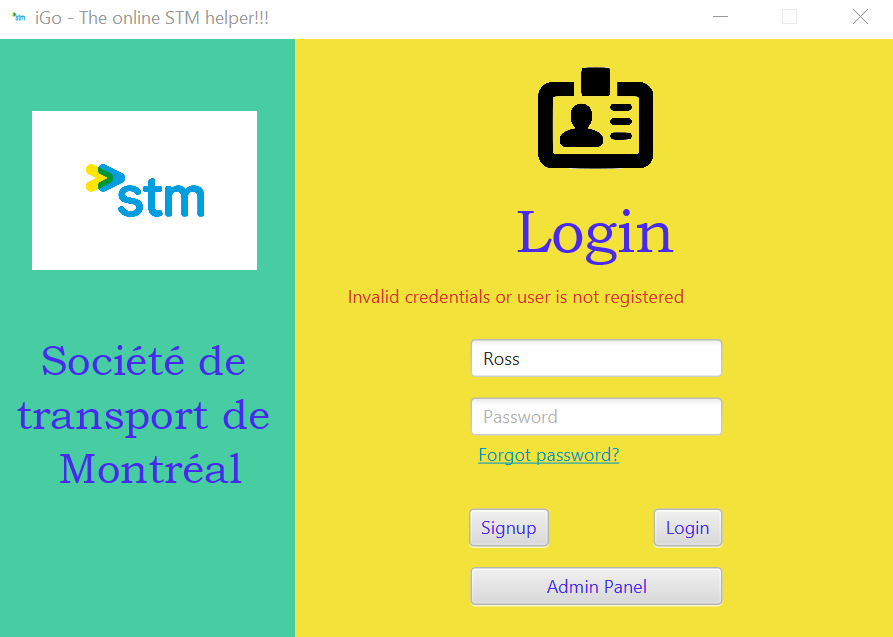
\includegraphics[width=\linewidth]{InvalidLoginCredentials.png}}
\caption{2. Registered user trying to log in with invalid credentials}
\end{center}

\begin{center}
  \makebox[\textwidth]{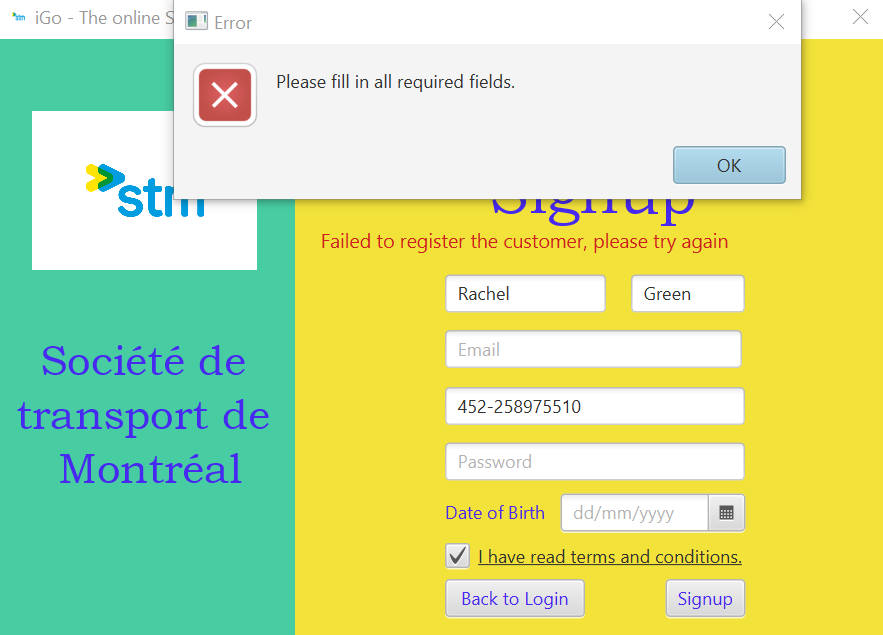
\includegraphics[width=\linewidth]{IncompleteSignupDetails.png}}
\caption{3. User trying to register with incomplete details}
\end{center}

\begin{center}
  \makebox[\textwidth]{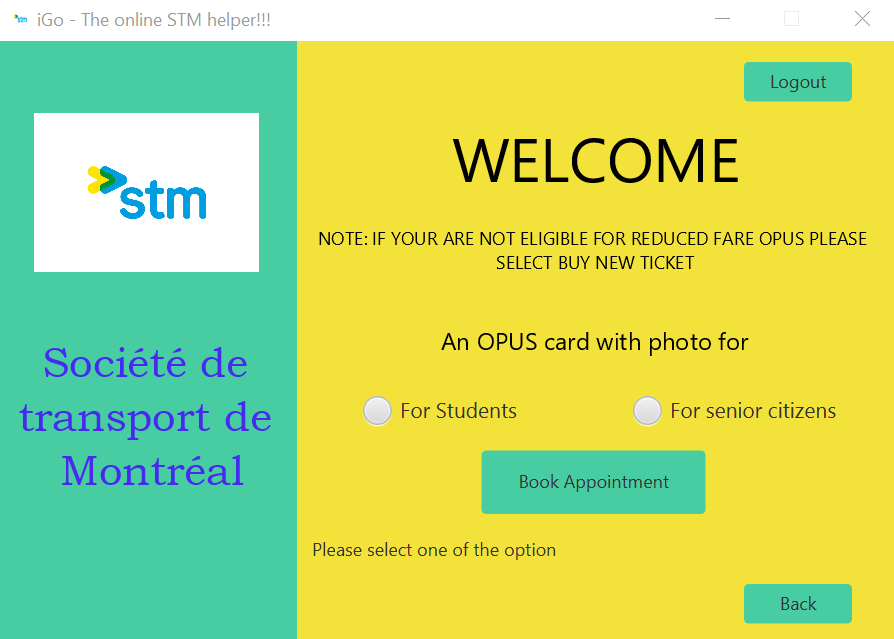
\includegraphics[width=\linewidth]{promptToSelectOption.png}}
\caption{4. User trying to book appointment without selecting option}
\end{center}

\begin{center}
  \makebox[\textwidth]{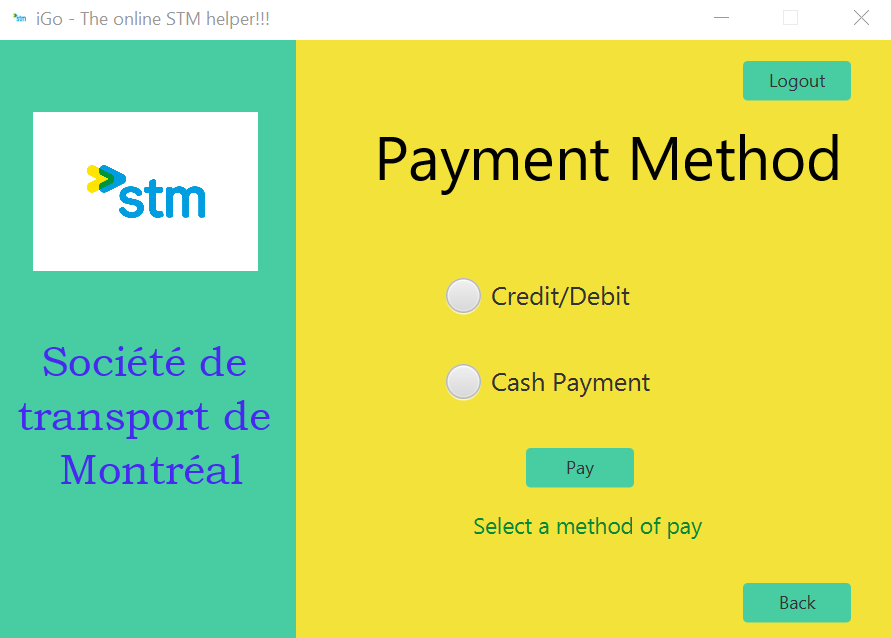
\includegraphics[width=\linewidth]{promptToSelectPayment.png}}
\caption{5. User trying to click pay without selecting payment method}
\end{center}

\newpage
\section*{References}
\begin{itemize}
    \item \href{https://www.ibm.com/docs/en/rsm/7.5.0?topic=structure-class-diagrams}{Structural Design Model}
    \item \href{https://www.microsoft.com/en-us/microsoft-365/business-insights-ideas/resources/guide-to-uml-diagramming-and-database-modeling}{UML Diagramming}
    \item \href{https://www.lucidchart.com/pages/uml-sequence-diagram}{Sequence Diagram}
\end{itemize}

\end{document}
